\chapter{Relaxation dynamics in a two-component system}

\section{Introduction}
Since the realization of superfluidity, quantum turbulence (QT) has been studied
in systems ranging from superfluid liquid
Helium~\cite{Barenghi2014, Walmsley2014} to quasi-particle
condensates in solid-state systems~\cite{Kreil2018}.
Due to their unprecedented experimental accessibility, QT in Bose-Einstein
condensates (BECs) in dilute, ultra-cold atomic gases have attracted considerable
theoretical~\cite{Kobayashi2007,Numasato2010, Reeves2013,
Billam2014,Simula2014,Baggaley2018} and
experimental~\cite{Henn2009,Kwon2014,Seo2017,Navon2019,Gauthier2019,
Johnstone2019} interest in both 2D and 3D configurations.
In a scalar BEC, the QT state is made up of a large number of vortices with
quantised circulation.
The collective behaviour of the vortices plays a key role
in the hydrodynamics, recovering features of classical turbulence that can
exhibit the characteristic Kolmogorov power-law spectrum~\cite{Kobayashi2005}.


In contrast to the scalar superfluids, multi-component and spinor BECs are
described by multi-component order parameters and allow for a wider range of
topological defects, which give rise to novel dynamics~\cite{Kasamatsu2016,
Weiss2019,Kobayashi2009,Kasamatsu2005}.
Consequently, there has been increasing interest in the properties of QT and
non-equilibrium dynamics in such
systems~\cite{Salman2009, Schmied2019, Karl2013, Prufer2018, Hofmann2014}.
The simplest non-scalar topological excitation appears in a two-component BEC,
described by two complex fields, as the appearance of a phase singularity in
only one component. 
When the atomic mass and mean density of the components are equal, such vortices
are often referred to as half-quantum vortices (HQVs), due to their similarities
with vortices carrying half a quantum of superfluid circulation in superfluid
\(^3\)He~\cite{Autti2016} and spin-1 BECs~\cite{Leonhardt2000,Seo2015}.
The study of QT in BECs can be separated into two distinct categories: 1.\
forced turbulence where a statistically stationary state is established;
2.\ decaying turbulence where a non-equilibrium initial condition, typically
involving vortices, relaxes towards equilibrium. 

As we have seen \textcolor{red}{IN RELEVANT PART}, the two-component BEC can be 
treated as a pseudospin-1/2 system. 
This new system gives rise to novel defects such as a half-quantum vortex 
otherwise unseen in a scalar condensate. 
In this chapter, we investigate the relaxation dynamics of half-quantum vortices 
(HQVs) in a two-dimensional, two-component condensate. 
Our interest is in studying the scaling laws that govern the decay rate of the 
vortices, and consequently the growth of the length scales associated with 
domains in the system, whilst varying the ratio of inter- to intra-species 
interactions. 
We study these scales by starting from an initially turbulent state containing
HQVs and subsequently letting the system relax in time.
Upon relaxation, vortices will annihilate leading to domain growth within 
the system.
To extract the appropriate length scales of these domains, we construct 
correlation functions, originally defined for an antiferromagnetic spin-1 
system~\cite{Symes2017}, which then allow us to extract relevant length scales
associated with spin and mass order.
By investigating these length scales temporally, we reveal interesting, 
novel dynamics occurring at early times for a sufficiently high ratio of 
inter- to intra-species interactions. 
This result is then confirmed by considering the total vortex number of the 
system. 
Furthermore, we contrast our observations for this system with similar
simulations that have been performed for scalar BECs and reported
in~\cite{Schole2012, Nowak2012, Karl2017}.
Finally, we discuss how our observations of anomalous vortex decay can be
explained by relating to previous work~\cite{Eto2011, Kasamatsu2016}.


\section{Two-component BEC as a pseudospinor}

\subsection{Easy-plane polar phase}\label{subsec:easy-plane-polar-phase}
The two-component BEC can be regarded as a `pseudospin-1/2' system as it can be
mapped directly to a certain configuration of the spin-1 condensate.
Recall that the spin-1 condensate with polar interactions \((c_2 > 0)\) supports a
polar ground state with \(|\vb{F}|=0\).
This state can be categorized in two different ways depending on the orientation
of the nematic director.
The first consists of the nematic director being aligned with the \( z \)-axis,
which is referred to as the easy-axis polar (EAP) phase.
This phase is stable for \( p=0 \) and \( q>0 \)
\textcolor{red}{See relevant section?}.
The second case consists of the director being in the \( xy \)-plane, which is
referred to as the easy-plane polar (EPP) phase.
This phase is stable for \( p=0 \) and \( q < 0 \).
The representative wavefunction for the EPP phase can be written as
\begin{equation}
    \psi_\mathrm{EPP} = \frac{1}{\sqrt{2}}\begin{pmatrix}
        1 \\ 0 \\ 1
    \end{pmatrix}.
    \label{eq:EPP_wavefunction}
\end{equation}
Since the middle component is empty, we can map this spinor directly onto a
two-component system.

\subsection{Mapping the EPP phase onto a two-component system}\label{subsec:mapping-the-epp-phase-onto-a-two-component-system}
To begin the mapping procedure, we first construct the time-independent
GPEs for the spin-1 system with a wavefunction that assumes an empty middle
component:
\begin{equation}
    \begin{aligned}
        \left[-\frac{\hbar^2\nabla^2}{2M}
        + (c_0 + c_2)|\psi_1|^2 + (c_0 - c_2)|\psi_{-1}|^2 
        + q - \mu\right]\psi_1 &= 0, \\
        \left[-\frac{\hbar^2\nabla^2}{2M}
        + (c_0 + c_2)|\psi_{-1}|^2 + (c_0 - c_2)|\psi_1|^2 
        + q - \mu\right]\psi_{-1} &= 0,
    \end{aligned}
    \label{eq:EPP-time-independent-GPEs}
\end{equation}
where \( \mu \) is the chemical potential of the system, and we have taken
\( p=0 \).

Similarly, the time-independent GPEs for the two-component system are
\begin{equation}
    \begin{aligned}
        \left(-\frac{\hbar^2\nabla^2}{2m_1} + g_1|\psi_1|^2
        +g_{12}|\psi_2|^2 - \mu_1\right)\psi_1 &= 0, \\
        \left(-\frac{\hbar^2\nabla^2}{2m_2} + g_2|\psi_2|^2
        +g_{12}|\psi_1|^2 - \mu_2\right)\psi_2 &= 0.
    \end{aligned}
    \label{eq:two-comp-time-independent-gpes}
\end{equation}
Using these time-independent equations, we can map the two-component system
to that of the spin-1 by comparing the coefficients with
Eq.~\eqref{eq:EPP-time-independent-GPEs}.
By doing this we find
\begin{equation}
    g_1=g_2=c_0+c_2, \enskip g_{12} = c_0-c_2, \enskip \mu_1=\mu_2=\tilde{\mu}, 
    \enskip m_1=m_2=M,
\end{equation}
where \( \tilde{\mu} = \mu - q \).
This directly relates the two-component BEC to the EPP phase of a spin-1
condensate.
Note that this mapping only holds when the interspecies interactions, chemical
potentials and masses of the atomic species in the two-component BEC are equal.
\textcolor{red}{Links to papers that discuss this particular type of
two-component BEC?}


\section{Half-quantum vortices in spin-1/2}
The pseudospinor nature of the two-component system allows for a novel vortex
structure otherwise unseen in scalar BECs.
To construct such a vortex, we start by defining the pseudospin-1/2
wavefunction:
\begin{equation}
    \mqty(\psi_1 \\ \psi_2) = 
    \mqty(|\psi_1|e^{i\theta_1} \\ |\psi_2|e^{i\theta_2}) = 
    e^{i\Theta}\mqty(|\psi_1|e^{i\Phi} \\ |\psi_2|e^{-i\Phi}),
    \label{eq:pseudospin-1/2-wavefunction}  
\end{equation}
where \( \theta_j=\mathrm{Arg}(\psi_j) \) for \( j=1,2 \) and
\begin{equation}
    \Theta = \frac{\theta_1 + \theta_2}{2}, \enskip 
    \Phi = \frac{\theta_1 - \theta_2}{2}.
    \label{eq:Theta-Phi}
\end{equation}
Gradients in \( \Theta \) are associated with a total, superfluid mass current
whereas gradients in \( \Phi \) are associated with pseudospin currents.
\textcolor{red}{Do I want to elaborate on this further? Potentially by looking
at actual expressions for mass and pseudospin current in two-component BECs.}
Now consider a vortex state which consists of a phase singularity in the
\(\psi_1 \) component such that about the singularity \( \theta_1 \) winds by
\( 2\pi \) and \( \theta_2 \) remains unchanged, i.e.\ it is a smooth phase
field.
Such a state can be written as
\begin{equation}
    \twovec{\psi_1}{\psi_2} 
    = \twovec{|\psi_1|e^{i\varphi}}{|\psi_2|}
    = e^{\varphi/2}\twovec{|\psi_1|e^{i\varphi/2}}{|\psi_2|e^{-i\varphi/2}},
\end{equation}
where \( \varphi \) is the azimuthal angle around the vortex core.
By comparing the above to Eq.~\eqref{eq:pseudospin-1/2-wavefunction}, we have
\( \Theta=\Phi=\varphi/2 \).
Using the fact the velocity is related to phase \(\vb{v}=\hbar/m\grad\Theta \),
the circulation is then given by
\begin{equation}
    \oint_C\vb{v}\cdot d\vb{\ell} = q\frac{\kappa}{2},
\end{equation}
where \( q \) denotes the charge of the vortex and \(\kappa=\hbar/m\) is the
quantum of circulation.
Traversing a point about the vortex shows the circulation is quantised in units
of \(\kappa/2\), half the usual circulation of \( U(1) \) vortices in scalar
BECs [REFs?].
Since this vortex carries half the circulation of a \( U(1) \) vortex, such a
vortex state is referred to as a half-quantum vortex\footnote{This vortex is 
topologically distinct from HQVs that arise in the A and polar phases of
superfluid \(^3\)He~\cite{Autti2016} and the polar phase of spin-1
BECs~\cite{Leonhardt2000, Seo2015}.}.

\section{Half-quantum vortex relaxation dynamics}
To begin studying the relaxation dynamics of HQVs in a turbulent system, we
numerically solve the two-component Gross-Pitaevskii equations in dimensionless
form
(\textcolor{red}{see Appendix for details of dimensionless form}):
\begin{equation}
    \begin{aligned}
        i\frac{\partial \psi_1}{\partial t} &= (-\nabla^2 + g|\psi_1|^2
        + \gamma|\psi_2|^2)\psi_1, \\
        i\frac{\partial \psi_2}{\partial t} &= (-\nabla^2 + g|\psi_2|^2
        + \gamma|\psi_1|^2)\psi_2.
    \end{aligned}
    \label{eq:dimensionless-two-comp-GPEs}
\end{equation}
where we have assumed each component has the same atomic mass and inter-species
interaction strength.
The key parameter is the ratio of inter- to intra-species interaction
\begin{equation}
    \gamma = \frac{g_{12}}{g}.
\end{equation}
We consider the case \(0 < \gamma < 1\) with all interactions repulsive such that
the condensate is stable against the separation of the components.

The inter- and intra-component interactions give rise to two important length
scales within the system.
These are, respectively, associated with variations in the total superfluid
density and the difference in density between the components.
The density and spin healing lengths are then defined as~\cite{Eto2011}
\begin{equation}
    \xi_d = \frac{\hbar}{\sqrt{2mgn_0}}, \qquad 
    \xi_s = \xi_d \sqrt{\frac{1 + \gamma}{1 - \gamma}},
    \label{eq:healing-lengths}
\end{equation}
where \(n_0\) is the background number density of each component in a uniform
system.
The size of the HQV core can be understood from the energetic hierarchy of
these healing lengths.
Since an HQV consists of a phase singularity in one component and not the other,
the core is free to fill with the atoms of the other component.
This corresponds to spatial variations in the \( z \)-component of the
pseudospin, the size of which is set by the spin healing length, \(\xi_s\).
The vortex core can expand when \(\xi_s \lesssim \xi_d\), which lowers
the total energy.
We see from Eq.~\eqref{eq:healing-lengths} that \(\gamma \) directly determines
the core sizes within our systems.
Similar energetic hierarchies exist in spinor BECs, which can facilitate
deformations of vortex cores such as the splitting of singly quantized vortices
into fractional vortices [REFS].

\subsection{Numerical setup}\label{sec:numerical-setup}
We solve Eq.~\eqref{eq:dimensionless-two-comp-GPEs} on a periodic domain with 
\(N_s^2=1024^2\) grid points which has dimensionless area \(L^2=N_s^2\) with
side length \(L=N_s\).
We take \(N=3.2\times10^9\) atoms per component and fix dimensionless
\(g=L^2/4N\).
The dimensionless density healing length is then fixed at
\(\xi_d=N_s/\sqrt{gN}=2\) in our system.
We wish to explore the effect of the inter-component interaction by varying
\(\gamma \) within the range \(0 < \gamma < 1\).

The initial state is constructed as follows.
We wish to construct \(48^2\) vortices in each component.
To do this we start with a grid of vortex positions such that the 
\(i\)-th vortex is to be imprinted at position \((x_i, y_i)\).
We repeat the same procedure for the other component.
However, to avoid overlapping vortex positions, we offset this grid in both
\(x\) and \(y\) whilst preserving the grid structure.
To facilitate a random distribution of vortices and subsequently turbulent
dynamics, we then displace each position by some small amount 
\((x_i, y_i) \rightarrow (x_i \delta + x_i, y_i + \delta y_i)\), where 
\(\delta x_i, \delta y_i < 3\xi_d\).
The vortices are then constructed as an alternating \( 2\pi \) winding of the
component phase about each vortex position using the method described
in~\cite{Billam2014}.
We imprint the vortices using a short imaginary time propagation of
Eq.~\eqref{eq:dimensionless-two-comp-GPEs} whilst keeping the phase profile
fixed to not alter the positions of the vortices.
This results in an initially turbulent system of HQVs.
The HQV cores correspond to a density depletion in one component at the position
of the phase singularity with a corresponding density peak at the same position
in the other component (see Fig.~\ref{fig:initial-vortex-state}).
\begin{figure}
    \centering
    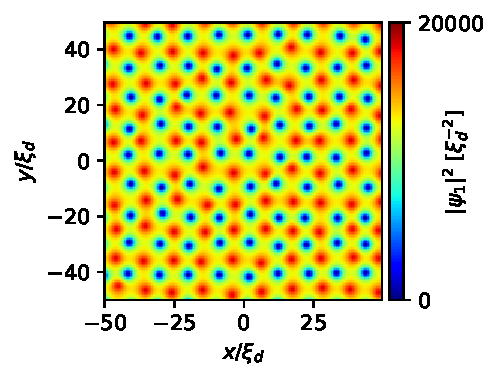
\includegraphics{gfx/ch-twoCompDynamics/init_state.pdf}
    \caption{Density of \(\psi_1 \) component in a \(100\xi_d\times100\xi_d\)
    subregion of the initial state after imaginary time propagation.
    We see the HQVs in this component by the density depletion.
    The density peaks correspond to the location of HQV cores in the other
    component, which have been filled by atoms in this
    component.\label{fig:initial-vortex-state}}
\end{figure}
Previous work has shown that clustering of vortices can lead to anomalously
slow coarsening dynamics~\cite{Karl2017} and thus constructing the initial
state this way ensures that there is no clustering of like-signed vortices.
From this initial state, the system evolves according to
Eq.~\eqref{eq:dimensionless-two-comp-GPEs}.
Two HQVs in the same component with opposite winding can annihilate, leading to
a decay of the total vortex number within the system.

\subsection{Interaction dependence of HQV core size}
We first investigate how \(\gamma \) affects the HQVs within our systems.
\begin{figure}
    \centering
    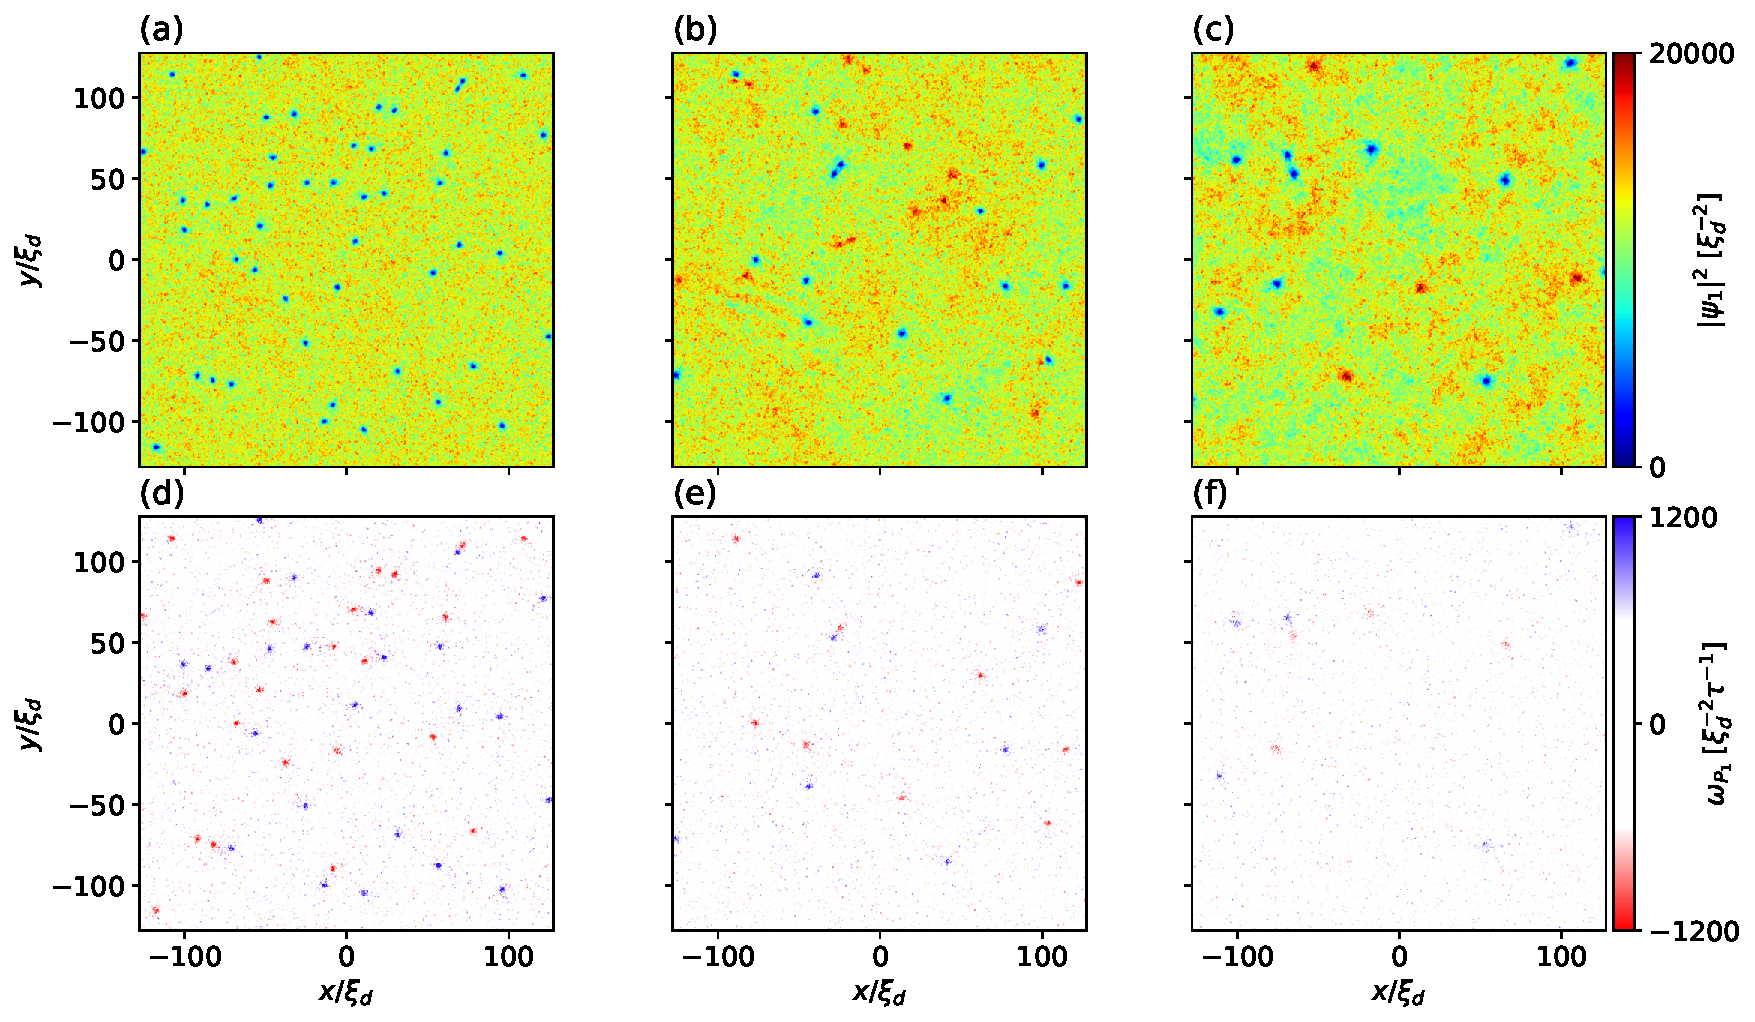
\includegraphics[width=\textwidth]{gfx/ch-twoCompDynamics/densVort.pdf}
    \caption{Density (a)- (c) and pseudo-vorticity (d)- (f) of the \(\psi_1 \)
    component in a \(256\xi_d \times 256\xi_d\) subregion at a time 
    \(t/\tau=2.5\times 10^4\xi_d^2\) for \(\gamma=0.1\) (left),
    \(\gamma=0.6\) (middle), and \(\gamma=0.8\) (right).
    The density depletions correspond to HQVs in this component.
    For \(\gamma \gtrsim 0.6\), density peaks reveal the locations of HQVs with
    the phase singularity in the other component where the cores have filled
    with atoms in this component.
    Vortices with positive (blue) and negative (red) circulation are
    identifiable in the pseudo-vorticity field.\label{fig:density-pseudo-vort}}
\end{figure}
Fig.~\ref{fig:density-pseudo-vort} shows the density field of the \(\psi_1 \)
component for \(\gamma = 0.1, 0.6, 0.8\).
One sees that as \(\gamma \) increases, the core size (i.e., the radial size of
the density depletion) also increases.
From Eq.~\eqref{eq:healing-lengths} we see that the size of the HQV core is
dependent on \(\gamma \), where \(\xi_s \rightarrow \xi_d\) as
\(\gamma \rightarrow 0\).
The healing lengths can explain why, for \(\gamma \geq 0.6\), bright density
peaks also appear within the \(\psi_1 \) field.
For small \(\gamma \), the density and spin healing lengths become comparable,
\(\xi_d \sim \xi_s\).
However, an increasing \(\gamma \) implies a larger spin healing length.
Consequently, atoms of the other component will fill the vortex core as the
resulting lowering of the kinetic energy offsets the cost of interaction energy.
This results in the expansion of the vortex cores to the size of the spin
healing length.
Hence, bright density peaks in Fig.~\ref{fig:density-pseudo-vort} correspond to
atoms in the \(\psi_1 \) component that has filled the core of an HQV in the
\(\psi_2\) component. \par
We can accurately track the positions of the HQVs in the system through
the pseudo-vorticity [REFS]
\begin{equation}
    \omega_\mathrm{p_j} = \frac{1}{2}\nabla \times {(n\vb{v})}_j,
\end{equation}
where
\begin{equation}
    {(n\vb{v})}_j = -i\left[\psi_j^*(\nabla\psi_j) - (\nabla_j^*)\psi_j\right]
\end{equation}
is the mass current of component \(j=1, 2\).
The pseudo-vorticity has the unique property of remaining regular and non-zero
within the vortex cores. On length scales greater than the spin healing length
away from a vortex core, the pseudo-vorticity quickly relaxes to zero as seen
in Fig.~\ref{fig:density-pseudo-vort} (d)- (f).
The sign of the pseudo-vorticity also determines the charge of the vortex.

\subsection{Investigating the kinetic energy spectrum}
A useful property to investigate in turbulent systems is the kinetic energy
spectrum [REFS?].
This spectrum provides useful insights into the spatial aspects of the
relaxation dynamics.
We start with the kinetic energy of the two-component system which is written
in terms of the density \(n_j\) and velocity \(\vb{v}_j\) of the \(j\)-th
component (\( j=1,2 \)) as
\begin{equation}
    E_\mathrm{kin} = \int d^2\vb{x} (|\nabla\sqrt{n_1}|^2 
    + |\nabla\sqrt{n_2}|^2)
    + \frac{1}{4}\int d^2\vb{x} (|\sqrt{n_1}\vb{v}_1|^2 
    + |\sqrt{n_2}\vb{v}_2|^2).
\end{equation}
The kinetic energy can be further decomposed into quantum pressure
(\( E^q\)) and a classical velocity (\(E^v\)) contributions:
\begin{equation}
    E^v = \frac{1}{4}\int d^2\vb{x} (|\sqrt{n_1}\vb{v}_1|^2 
    + |\sqrt{n_2}\vb{v}_2|^2),
\end{equation}
\begin{equation}
    E^q = \int d^2\vb{x} (|\nabla\sqrt{n_1}|^2 
    + |\nabla\sqrt{n_2}|^2).
\end{equation}

To extract energy spectra from these contributions, we define the generalized
velocities for the incompressible (i), compressible (c), and quantum pressure
(q) parts as
\begin{equation}
    \begin{aligned}
        \vb{w}^{i, c} &= \sqrt{n_1}\vb{v}_1^{i, c} + \sqrt{n_1}\vb{v}_1^{i, c}
        \\
        \vb{w}^q &= 2 (\nabla \sqrt{n_1} + \nabla \sqrt{n_2}).
    \end{aligned}
\end{equation}
Here, the incompressible and compressible parts of the velocity field are
extracted from a Helmholtz decomposition [REF] which splits the velocity into a 
divergence-free incompressible part, \(\nabla \cdot \vb{v}^i = 0\), and an 
irrotational, compressible part, \(\nabla \times \vb{v}^c=\vb{0}\).
Hence, in Fourier space, the kinetic energy spectrum can be calculated by
taking the Fourier transform of the generalized velocities and integrating over
the \(k\)-space angle as
\begin{equation}
    E^\delta(k) = \frac{1}{4} \int_{0}^{2\pi} d\Omega_k
    |\tilde{\vb{w}}^\delta(\vb{k})|^2
    \qquad (\delta = i, c, q),
\end{equation}
for wave number \(k=|\vb{k}|\).
The total kinetic energy is then given by the sum of each contribution,
integrated over all \(k\)
\begin{equation}
    E_\mathrm{kin} = \sum_\delta \int dk E^\delta (k) \qquad (\delta = i, c, q).
\end{equation}
The occupation numbers of each contribution are extracted as
\begin{equation}
    n^\delta(k) = k^{-2}E^\delta(k) \qquad (\delta = i, c, q).
\end{equation}
Finally, the total occupation number of the system is given as
\begin{equation}
    n(k) = \int_{0}^{2\pi} d\Omega_k \psi_1^*(k)\psi_1(k) 
    + \psi_2^*(k)\psi_2(k).
\end{equation}

\begin{figure}[t!]
    \centering
    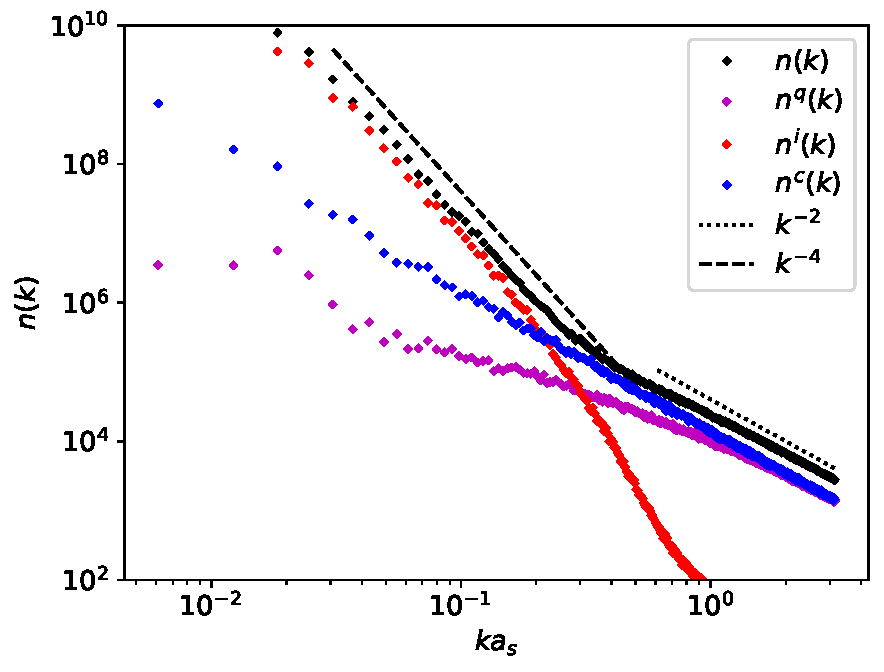
\includegraphics[scale=0.75]{gfx/ch-twoCompDynamics/spectra.pdf}
    \caption{Occupation numbers for the quantum pressure (purple diamonds),
    incompressible (red diamonds), and compressible (blue diamonds)
    contributions for \(\gamma=0.6\).
    The total occupation number (black diamonds) is obtained from the sum of
    each contribution.
    The total occupation number has two distinct scalings: a \(k^{-2}\) 
    (dotted line) in the ultra-violet region, and a \(k^{-4}\) scaling
    (dashed line) in the infrared.\label{fig:kinetic-energy-spectra}}
\end{figure}
We plot the occupation number for each energy contribution, as well as total
occupation number, at a late time for \(\gamma=0.6\) in
Fig.~\ref{fig:kinetic-energy-spectra}.
The total occupation number exhibits two different scalings: A \(k^{-4}\) in the
ultraviolet (UV), and \(k^{-2}\) in the infrared (IR). 
The same scalings have been found in some 2D, turbulent, scalar BEC systems
containing scalar vortices [REFS].
The decomposition of the kinetic energy into its respective contributions
allows us to see that the incompressible contribution dominates the spectrum
in the IR region, and is therefore responsible for the transition to the
\(k^{-4}\) scaling.
This incompressible contribution is directly associated with the vortices in
the system. \textcolor{red}{Elaborate? Why exactly?}
Similarly, we see it is both the compressible and quantum pressure contributions
that dominate in the UV region, facilitating the transition to the \(k^{-2}\)
scaling.
This \(k^{-2}\) scaling is characteristic of weak-wave turbulence [REFS].

This scaling of the kinetic energy was observed throughout all values of
\(\gamma \) tested, indicating that it is quantitatively insensitive to variations
in \(\gamma \).
The investigation into the kinetic energy spectrum reveals that \(\gamma \) has
negligible effects on the spatial aspects of the relaxation dynamics, and shows
quantitatively similar behaviour to some turbulent scalar BEC systems
containing scalar vortices.

\subsection{Spin spectra?}

\subsection{Temporal aspects of decay}
To measure the temporal aspect of the relaxation dynamics, we wish to
construct correlation functions.
Since our pseudo-spinor order parameter is composed of a mass part and a spin
part (c.f. Eq.~\eqref{eq:Theta-Phi}), it is natural to then construct both a
mass and spin correlation function.\par
To begin, we need to identify appropriate quantities that serve as order
parameters for our system.
By taking motivation from the EPP phase in spinor BECs, one such quantity is
the planar tensor~\cite{Symes2017}
\begin{equation}
    \mathsf{Q} = \mqty(Q_{xx} & Q_{xy} \\ Q_{xy} & -Q_{xx}),
\end{equation}
where \(Q_{xx} = \mathrm{Re}(\psi_1^*\psi_2)\) and
\(Q_{xx} = \mathrm{Im}(\psi_1^*\psi_2)\), showing this quantity depends on the
relative phase coherence of the two components.
The eigenvalues of \(\mathsf{Q}\) are given by
\{ \(-\frac{1}{2}|\alpha|, \frac{1}{2}|\alpha|\) \}, where
\(\alpha=-2\psi_1\psi_2\).
If we consider the general wavefunction defined in
Eq.~\eqref{eq:pseudospin-1/2-wavefunction}, then evaluating \(\mathsf{Q}\) and
\(\alpha \) gives
\begin{equation}
    Q_{xx} = |\psi_1||\psi_2|\cos({2\Phi}), \qquad 
    Q_{xy} = -|\psi_1||\psi_2|\sin({2\Phi}),
\end{equation}
\begin{equation}
    \alpha = -2|\psi_1||\psi_2|e^{2i\Theta}.
\end{equation}
This shows that \(\mathsf{Q}\) is sensitive to the phase of the spin,
\( \Phi \), whereas \(\alpha \) is dependent upon the global phase,
\( \Theta \).

Armed with these quantities, we can then construct correlation functions related
to the mass and spin parts of our pseudo-spinor order parameter.
These are defined, respectively, as
\begin{equation}
    G_\Theta = \frac{1}{n^2}\langle \alpha^*(\vb{0})\alpha(\vb{r}) \rangle,
\end{equation}
\begin{equation}
    G_\Phi(\vb{r}, t) = 
    \frac{2}{n^2}\mathrm{Tr}
    [\langle \mathsf{Q}(\vb{0})\mathsf{Q}(\vb{r})\rangle],
\end{equation}
where \( \langle \cdot \rangle \) denotes ensemble averaging.
By exploiting the fact that our system is homogeneous, we can replace ensemble
averages with spatial averages.
To obtain the 1D spectrum, we perform an angular integration in k-space.
The spin correlation function is then computed as
\begin{equation}
    G_\Phi(r, t) = \int d\Omega_k \int \frac{d^2\vb{x}'}{L^2}
    \frac{2}{n^2}\mathrm{Tr}
    [\langle \mathsf{Q}(\vb{x'})\mathsf{Q}(\vb{x}' + \vb{r})\rangle],
\end{equation}
where \(\int d\Omega_k\) denotes integration over the k-space angle, whilst
\(\int d^2\vb{x}'/L^2\) is spatial averaging.
We perform the same averaging for the mass correlation function.

\begin{figure}
    \begin{subfigure}{\textwidth}
        \centering
        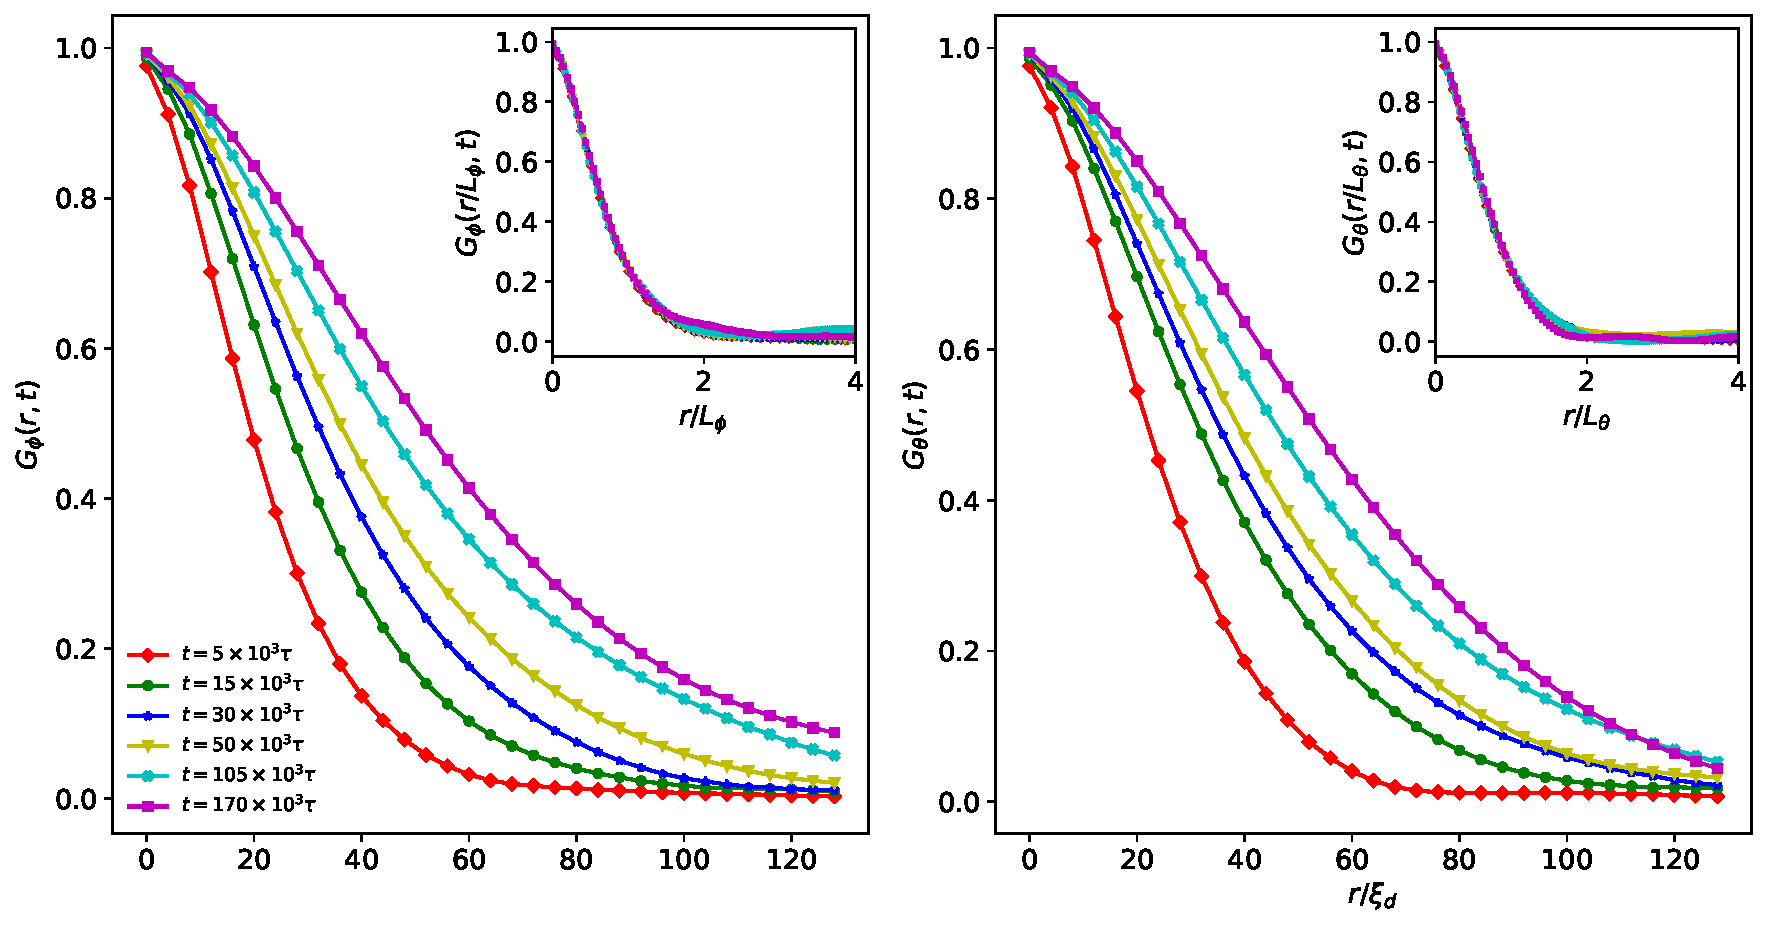
\includegraphics[width=\textwidth]{
            gfx/ch-twoCompDynamics/correlations.pdf}
        \caption{\label{fig:correlation-functions}}
    \end{subfigure}\\
    \begin{subfigure}{0.5\textwidth}
        \centering
        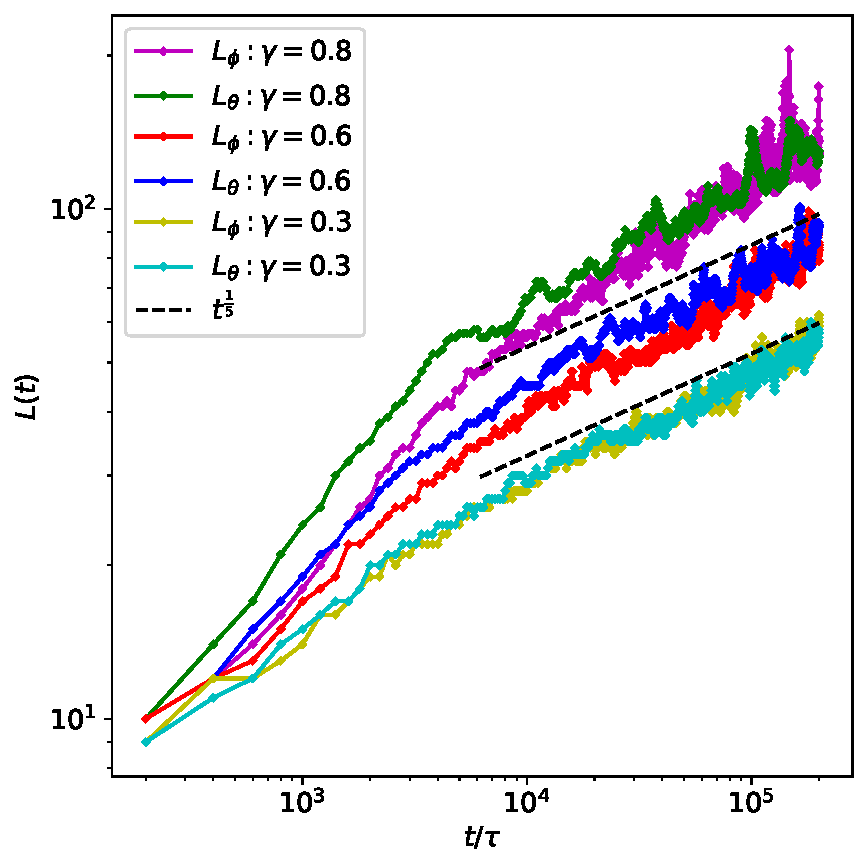
\includegraphics[width=\textwidth]{
            gfx/ch-twoCompDynamics/correlation_lengths.pdf}
        \caption{\label{fig:correlation-lengths}}
    \end{subfigure}
    \begin{subfigure}{0.5\textwidth}
        \centering
        \includegraphics[width=0.8\textwidth]{example-image-a}
        \caption{\label{fig:scalar-vortex-lengths}}
    \end{subfigure}
    \caption{}
\end{figure}
Fig.~\ref{fig:correlation-functions} shows both correlation functions for
\(\gamma=0.6\) for various times through the simulation.
We see that as time increases, the correlation functions extend over larger
distances which indicates that the respective domains are growing over time,
showing long-range order is being established.

From these correlation functions, we may extract a correlation length,
\(L_\delta \) with \(\delta \in \{\Theta, \Phi \} \), that enables us to
determine a length scale over which the correlation function decays.
We take the correlation length to be the value at which the corresponding
correlation function decays to a quarter of its value at
\(r=0\): \(G_\delta(L_\delta, t) = \frac{1}{4}G_\delta(0, t)\).
Using the correlation length, we can determine whether the correlation functions
exhibit dynamical scaling, which implies the form of the functions remains
self-similar at different times throughout the simulation.
This means the function collapses to a universal, time-independent function
when scaled by the correlation length: \(H_\delta(r) = G(r/L_\delta(t), t)\).
The insets of Fig.~\ref{fig:correlation-functions} show the scaling of the
correlation functions when scaled by the respective correlation length.
This confirms that the correlation functions within our system do exhibit
dynamical scaling. \textcolor{red}{Reference to other systems where dynamical
scaling is also seen?} \par
Fig.~\ref{fig:correlation-lengths} shows the correlation lengths for
\(\gamma=0.3\), \(\gamma=0.6\), and \(\gamma=0.8\) as functions of time.
We see that at late times in the evolution, all correlation lengths tend to a
universal \(t^\frac{1}{5}\) scaling.
However, the early-time dynamics are remarkably different for the various
\(\gamma \).
As \(\gamma \) increases, there is a faster growth of the correlation lengths at
early times, which signifies the correlation length being \(\gamma \)-dependent.
\par
We investigate this behaviour by considering the total vortex number of
the system as a function of time.
We can then extract the mean distance between the vortices as
\(\ell_d=1/\sqrt{N_\mathrm{vort}}\), where \(N_\mathrm{vort}\) is the total
number of vortices in the two components.
In a scalar BEC containing an initially large number of vortices, it has been
observed that \(\ell_d \sim t^\beta \)~\cite{Karl2017}, where \(\beta \)
characterizes the annihilation rate of vortices.
In particular, there were two scaling observed: Firstly, a \(\beta=1/5\) scaling
after some short period of evolution.
This scaling is included in Fig.~\ref{fig:correlation-lengths} as a comparison.
Secondly, after a much longer period of evolution, a \(\beta=1/2\) scaling
emerges.
This second scaling can be delayed if the initial vortex distribution is
highly clustered~\cite{Karl2017}.
Fig.~\ref{fig:scalar-vortex-lengths} is a reproduction of both the early- and
late-time scaling of the mean vortex distance, \(\ell_d\), for a scalar system
using the parameters of~\cite{Karl2017}.
We consider three initial conditions: Firstly, we constructed a grid of vortices
analogous to our two-component system (see Sec.~\ref{sec:numerical-setup}).
Secondly, we considered a random distribution of vortices; one with noise
added to the energy spectrum, and one without.
We see that at early and intermediate times, there is a clear \(t^{1/5}\)
scaling in all of the initial states tested.
Furthermore, at late times we recover the \(t^{1/2}\) scaling for all initial
states.
This indicates the scaling is robust and insensitive to the initial conditions.
\par
Motivated by this previous work in scalar BECs, we conduct a similar analysis
on our two-component system containing HQVs, and determine how \(\gamma \)
affects the vortex decay rate.
In particular, we consider the early-time evolution in which
Fig.~\ref{fig:correlation-lengths} suggests interesting dynamics.
\begin{figure}
    \centering
    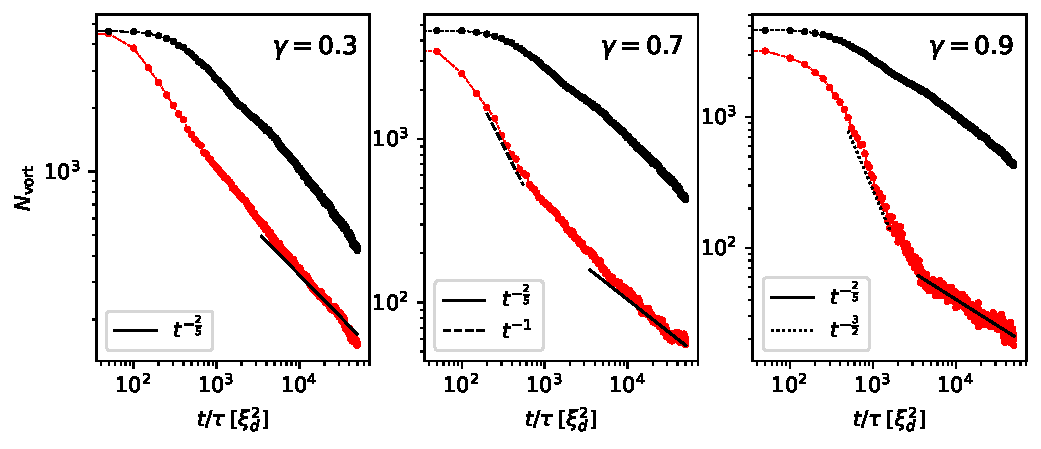
\includegraphics[width=\textwidth]{gfx/ch-twoCompDynamics/vortex_number.pdf}
    \caption{Total vortex number as a function of time for
    \(\gamma=0.3,0.7,0.9\) (red circles).
    Larger \(\gamma \) leads to a faster decay rate of vortices at
    early times due to the rapid annihilation of opposite-signed vortices
    within the same component.\label{fig:vortex-number}}
\end{figure}
The total vortex number is plotted in Fig.~\ref{fig:vortex-number} for
\(\gamma=0.3\), \(\gamma=0.7\), and \(\gamma=0.9\).
We see that for \(\gamma=0.3\), the vortex decay rate is mostly consistent
throughout the evolution, which tends to a \(t^{-2/5}\)
(\(\ell_d \sim t^{1/5}\)) scaling at later times.
More interesting dynamics are revealed for \(\gamma=0.7, 0.9\) where two
different scaling regimes emerge at early times
(\(2.5\times10^2\xi_d^2 \lesssim t/\tau \lesssim 2.5\times10^3\xi_d^2\)) with
\(N_\mathrm{vort} \sim t^{-1}\) for \(\gamma=0.7\) and
\(N_\mathrm{vort} \sim t^{-3/2}\) for \(\gamma=0.9\).
After the initial differing early-time dynamics, the systems then tend to a
universal \(t^{-2/5}\) scaling, which corresponds to \(\ell_d\sim t^{1/5}$
similar to the scalar BEC simulation shown.
These results show a better fit to the theoretical \(t^{1/5}\) scaling than 
indicated by the correlation lengths shown in
Fig.~\ref{fig:correlation-lengths}.
This further suggests that \(L_{\Phi,\Theta}\) differs slightly from \(\ell_d\),
even though the growth of the correlation lengths is driven by vortex
annihilation.
Fig.~\ref{fig:vortex-number} only extends up to \(t/\tau=5\times 10^4\xi_d^2$,
and we expect to see a universal transition to
\(N_\mathrm{vort}\sim t^{-1}\) (\(\ell_d\sim t^{1/2}\)) at much later times for
sufficiently small \(\gamma \).
For large \(\gamma \), due to the rapid annihilation of vortices at early times,
there may not be enough vortices left within the system to facilitate the
transition to the \(N_\mathrm{vort} \sim t^{-1}\) regime.
\par
We wish to investigate further the effect of \(\gamma \) on the initial decay
rate of the vortices.
We can model the vortex decay rate as a simple kinetic-like equation of the form
\begin{equation}
    \pdv{N_\mathrm{vort}}{t} \sim N_\mathrm{vort}^\eta,
\end{equation}
where \(\eta > 1\).
The form of this equation states that the decay rate of the vortices is
dependent on the total number of vortices facilitating the annihilation.
Using this simple model, we can extract a scaling for the total vortex
number as
\begin{equation}
    N_\mathrm{vort} \sim t^{-2/z},
    \label{eq:vortex-number-scaling}
\end{equation}
where \(z=-2(1-\eta)\).
An exponent of \(z=2\) corresponds to a two-body collision process, in which
only two vortices are required to annihilate.
On the contrary, an exponent of \(z=5\) corresponds to a three-body collision
process, where three vortices are necessary to facilitate annihilation.
\begin{figure}[t!]
    \centering
    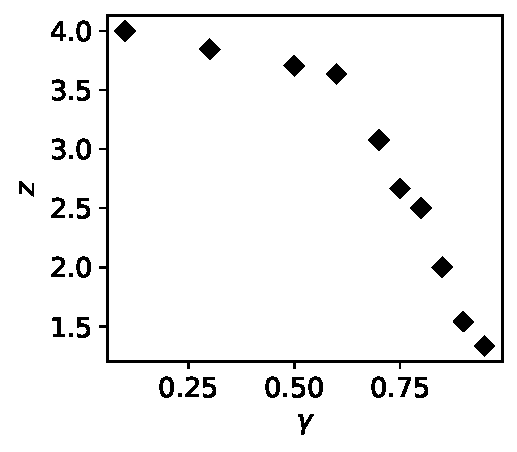
\includegraphics{gfx/ch-twoCompDynamics/gamma_vs_expo.pdf}
    \caption{The exponent \( z \) in Eq.~\eqref{eq:vortex-number-scaling} as a
    function of \(\gamma \).
    We see that after \(\gamma \gtrsim 0.6\) a rapid decrease of the exponent
    occurs, signalling a rapid change in vortex
    dynamics.\label{fig:exponent-vs-gamma}}
\end{figure}
Fig.~\ref{fig:exponent-vs-gamma} shows the exponent, \( z \), as a function of
\(\gamma \) where \( z \) is extracted within the time interval
\(2.5 \times 10^2\xi_d^2 < t/\tau < 2.5\times10^3\xi_d^2\).
We see a rapid decrease of the exponent after \(\gamma \gtrsim 0.6\), in which
Fig.~\ref{fig:vortex-number} shows the rapid annihilation of vortices is
prevalent.
The decrease of the exponent in our simulations signals an additional vortex
interaction mechanism not present in scalar BEC systems.

\subsection{HQV dipole dynamics}
Numerous studies have been conducted to try and understand the inter-vortex
forces between HQVs in two-component systems~\cite{Eto2011, Kasamatsu2016}.
In particular, Kasamatsu {\it et.\ al.}~\cite{Kasamatsu2016} tried to derive a
point vortex model to explain the dynamics shown in
Fig.~\ref{fig:exponent-vs-gamma} but found that the model failed to accurately
predict in vortex dynamics.
We can discern more about the dynamics of these HQVs by considering dipole
motion.


As a simple test case, I consider two HQVs of opposite winding within the same
component.
The vortices are placed in a uniform system
